%%%%%%%%%%%%%%%%%%%%%%%%%%%%%%%%%%%%%%%%%%%%%%%%%%%%%%%%%%%%%%%%%%%%%%
% How to use writeLaTeX: 
%
% You edit the source code here on the left, and the preview on the
% right shows you the result within a few seconds.
%
% Bookmark this page and share the URL with your co-authors. They can
% edit at the same time!
%
% You can upload figures, bibliographies, custom classes and
% styles using the files menu.
%
%%%%%%%%%%%%%%%%%%%%%%%%%%%%%%%%%%%%%%%%%%%%%%%%%%%%%%%%%%%%%%%%%%%%%%




\documentclass[12pt]{article}
% \usepackage{titlesec}

% \setcounter{secnumdepth}{4}

\usepackage{sbc-template}
\usepackage{enumitem}
\usepackage{graphicx,url}
%\usepackage{hyperref}
\usepackage{ntheorem}
\usepackage{xcolor}
\usepackage{color,soul}
\usepackage[utf8]{inputenc}  
% \documentclass[landscape, 12pt]{article}
% \usepackage[table, svgnames, dvipsnames]{xcolor}
% \usepackage{longtable}
% \usepackage[a4paper, landscape, margin=1cm,]{geometry}

\sloppy

\title{EduVizBR: A decision support system for \\ Brazilian students' performance analysis} 

\author{Chrystinne Fernandes\inst{1}, Diénert Vieira\inst{1}, Tassiane Barros\inst{1}, \\ Aian Shay\inst{1}, 
Nicksson Freitas\inst{2} and Tiago Vinuto\inst{2}}


\address{
    Centro de Informática -- Universidade Federal de Pernambuco (UFPE)\\
    Recife -- PE -- Brazil
\nextinstitute
  Samsung Development Institute for Informatics (SiDi)\\
  Recife -- PE -- Brazil
  \email{\{cof2, dav, mtbl, asbdc\}@cin.ufpe.br}
  \email{\{nicksson.a, t.vinuto\}@sidi.org.br}
}

\begin{document} 
%A decision support system to assist the analysis of factors that affect Brazilian students' academic performance%
\maketitle


\begin{abstract} 
% Refazer no final% 
Due to the explosive growth of educational data resulting from technological advances, Educational managers tend to be overwhelmed by the massive volume of data available during their decision-making process. 
As public datasets become available to be explored, more assistant tools are demanded to process, mine, and filter strategic knowledge into massive databases. Therefore, decision support tools are essential to help managers focus on the relevant subjects and gain the necessary knowledge to make faster and more reasonable decisions. 
In this paper, we present the EduVizBR, a decision support tool designed to assist Educational managers in analyzing the Brazilian students' performance at school. All the analyses are performed through the use of a robust dashboard containing selectable filters to interactively and quickly access the desired information. The EduVizBr allows managers to explore a massive volume of integrated educational data by narrowing their analyses according to: the most relevant impact factors presented in the literature, year of interest, and school subjects. We validated our tool through the conduction of a case study to analyse the school performance of high school students in the Brazilian national exam (ENEM). In this scenario, the EduVizBR was able to provide interesting insights about how gender impacts students' grades in all Brazilian states, and the influence of parents' educational attainment and parents' professions on their children's grades. Finally, we also analysed the trend for the students' performance over the last six years considering the mentioned factors.  

\end{abstract}


\section{Introduction} 
%Contexto/Problema%


The recent technological advances and easy access to the Internet contribute to the explosive growth of educational data. As public datasets become available to be explored, more assistant tools are demanded to process, mine, and filter strategic knowledge into massive databases  \cite{Terrin2014}. Educational Data Mining (EDM) is a research area that addresses different methods and tools that can be utilized for exploring the increasingly large-scale data that come from educational scenarios to better understand students and their context \cite{Romero2020}. Additionally, EDM has an emerging field named Educational Process Mining (EPM) aiming to make unexpressed knowledge explicit and to facilitate better understanding of the educational process \cite{Bogarn2017}.

%Problem/Proposta% 
Educational managers such as managers, coordinators, assistants, and professors
tend to be overwhelmed by the massive volume of data available during their decision-making process. Moreover, raw data does not provide the information needed to make accurate and agile decisions. Therefore, Decision Support Systems (DSS) are essential to help managers focus on the relevant subjects and gain the necessary knowledge to make faster and more reasonable decisions \cite{Velasco2020,RoqueeFaria2019}. In this process, consistent methods and approaches are required to
treat, group, and prepare all data in a single data warehouse.

%[RELACIONADOS E AS DESVANTAGENS]
Finding a set of factors that influence students' performance and that can be applied to a specific education scenario of investigation is a difficult task. This is mainly because the set of factors presented in the literature are too subjective to be measured through the available datasets in the field of education, such as: personal motivation, parents' expectations and involvement, home affective environment, discipline, and structure for learning. 
In this work, we investigated factors that affect students' performance in assessments worldwide, according to the literature. We found that these factors are mainly related to the social and economic context (e.g., student's sex, age, parents' level, parents' education, income, ethnicity, among others). The studies we found come mainly from areas such as psychology, representing surveys applied to the student population \cite{Farooq2012FACTORSAS, Stewart2007}. These works met their expecting results of finding the factors that influence students' performance, and present interesting analyses regarding the education scenario. However, as a drawback to these studies, we can point out the lack of any technological resource utilized to present their results through interactive data visualization tools.    

%[AQUI FALTA UM PARAGRAFO DESCREVENDO A IMPORTÂNCIA DE ENTENDER OS FATORES QUE IMPACTAM O REDIMENTO ESCOLAR (É IMPORTANTE REALÇAR O QUANTO SUA PROPOSTA É ÚTIL PARA ENCONTRAR E MONITORAR OS FATORES QUE IMPACTAM A EDUCAÇÃO)]%

In this work, we utilized these factors - collected from the literature -, as the main targets to generate data visualization in our system. By presenting data visualization according to these factors, we aim to assist educational managers to quickly find the most important information. In addition, we aim to validate if the factors presented in the literature as impacting students' performance in other countries also have a significant impact on Brazilian students.

%[Quais vantagens e Benefícios da Proposta? O que acontece se não tiver a proposta?]%
The main advantage of our solution is the decision support tool we provide to guide Education managers. Through the use of this system, managers have the flexibility to filter the most relevant information according to the factors, desired year (2015-2020), and even Brazilian states. We provide a robust dashboard containing selectable filters to quickly and interactively access the desired information.

%Objetivos%
The main goal of this work is the conception of a decision support tool designed to assist Education managers in analyzing Brazilian students' school performance. To validate our system, we conducted a case study to analyze the performance of high school students in the national exam (ENEM).
 
As the main contributions of our research project, we highlight: 

\begin{enumerate}
    \item The investigation and findings related to the factors that affect students’ performance in Brazil using six real datasets. We understand that other researchers can benefit from these results validating these factors with educational data from anywhere in the world;
    \item  A new pipeline to process, integrate and group different public datasets in Brazil, in our case, ENEM, FUNDEB and PNAE, including data preprocessing and many descriptive analyses available in this paper's repository; 
    \item The design and development of a decision support system for Educational Managers to make faster and more strategic decisions using interactive visualizations;
    \item The conduction of a use case comprising the exploitation and analysis of ENEM's datasets to validate our decision support tool.
    \item The EduVizBR assisted us in answering important research questions about Brazilian students' performance.
    
\end{enumerate}

%Como está organizado o paper%
This paper is organized as follows: Section 2 presents our related work, with studies describing strategies to deal with the problem of analysing students' performance according to the most relevant factors for the education scenario. In this section, we also discuss how these works are distinct from our approach. Section 3 presents the decision support tool application we built, with the architecture scheme containing the applications' modules, such as data input, preprocessing, visualization, and data analysis. Our main contributions are presented in Sections 3 and 4, where we describe our tool and discuss our main research question and sub-questions. Finally, we conclude this paper and present possible future work in Section 5.

\section{Related Work}\label{related}

In our search for related work, we gathered papers that could help us to identify the factors that affect student's performance. 

% (colocar trabalhos sobre sistemas de suporte a decisao) %

According to \cite{Lopes2020}, the Literature indicates that several aspects, internal and external to the school, can affect student performance in assessments. These aspects include the family, and classes or social strata. They can be divided into hierarchical levels organized into three distinct levels: i) at the student level, ii) at the class level, and iii) at the school level. The student level comprises personal and family aspects such as socio-demographic characteristics and family socioeconomic and cultural capital. The class level, on the other hand, is related to aspects of the classroom, such as teacher characteristics, peer effects, and pedagogical styles and practices. At last, the school level, encompasses factors related to the educational institution, such as violence, school policies or practices \cite{Lopes2020}.

The research carried out in \cite{chaia2017drives} analyzed the factors that influence the academic performance of students in the exam of the Programme for International Student Assessment (PISA). The study listed five factors that have the greatest impact on students' academic performance: i) personal motivation (mentality), ii) the proper combination of teacher guidance and self-research in teaching practice, iii) the use of information and communication technology (ICT) as a pedagogical tool by teachers, iv) the increase in school hours and v) early childhood education.

In \cite{alves2019decada}, the SAEB data, ranging from 2007 to 2017, was investigated to find out if there had been advances in the quality of Brazilian education in the last ten years. The authors analyzed students' learning and passing rate for elementary school. In addition, the work aimed to analyze the students' improvement, according to quality indicators such as regional or social characteristics. The results showed a continuous improvement of these indicators in all regions and social groups.

In \cite{Christenson_1992}, the authors present the following factors that influence students' achievement: i) parents' expectations and attributions, ii) parents' involvement,  iii) home affective environment, iv) discipline, and v) structure for learning. The latter means how the environment can be manipulated to encourage and support children’s academic learning. It includes homework, verbal interaction, presence of books and appropriate play materials, adult modeling of reading, and television viewing.

Another study \cite{Farooq2012FACTORSAS} was conducted to examine different factors influencing the academic performance of secondary school students in a metropolitan city of Pakistan. A survey was conducted by using a questionnaire for gathering information about different factors relating to academic performance of students. The respondents of the survey for this study were 600 10\textsuperscript{th} grade students (300 male and 300 female). The academic performance was measured by the result of their 9\textsuperscript{th} grade annual examination. Standard t-test and ANOVA were applied to investigate the effect of different factors on students’ achievement. The factors brought by this work were: i) age, ii) gender, iii) geographical belongingness, iv) ethnicity, v) marital status, vi) language, vii) parents’ educational level, viii) parental profession, ix) income, x) socioeconomic status (SES), and xi) religious affiliations. The findings of this study are the following: 

\begin{itemize}
    \item[\textbf{1.}] Socioeconomic status (SES) and parents’ education have a significant effect on students’ overall academic achievement as  well as achievement in the subjects of Mathematics and English;  
\end{itemize}

\begin{itemize}
    \item[\textbf{2.}] The high and average socioeconomic level affects the performance more than the lower level;  
\end{itemize}

\begin{itemize}
    \item[\textbf{3.}] Parents’ education means more than their occupation in relation to their children’s academic performance at school;
\end{itemize}

\begin{itemize}
    \item[\textbf{4.}] Girls perform better than the male students.    
\end{itemize}

In our work, we defined a set of eight factors based on the factors showed in the previous study \cite{Farooq2012FACTORSAS}. Additionally, we conducted our analysis based on the analysis made by \cite{Farooq2012FACTORSAS} to compare our results with those listed in their research.  

\section{EduVizBR} 

The EduVizBR tool was designed in a simple but functional way where three layers serve one another: Extract Transform and Load (ETL) Layer, Data Warehouse Layer and Data Visualization Layer. 


\subsection{Architecture}

In Figure \ref{data_flow} we present the architecture of our developed tool.

\begin{figure}[h!] 
\centering
\includegraphics[width=1\textwidth]{images/data_flow.jpg}
\caption{EduVizBR Architecture} 
\label{data_flow}
\end{figure}

The components and functioning of each layer are discussed below:


\paragraph{ETL Layer}\

The ETL layer gets raw input data from the three public datasets (i.e. ENEM, FUNDEB, and PNAE) we are using. It preprocesses, cleans, and transforms this data and selects what is necessary to our analysis, such as specific columns of interest, and removes rows with no information. After that, this tidied data is sent to the next layer (i.e., the Data Warehouse layer). In the ETL layer, we utilized the Pandas library for Exploratory Data Analysis (EDA), along with Dask for processing the massive volume of data.

\paragraph{Data Warehouse Layer}\

The job of the Data Warehouse Layer is to gather the cleared datasets from the ETL layer, performing a join on them, this way we could build relations between the three different datasets.  It also stores this unified version from our initial datasets in a way that is ready to be sent to the next layer (i.e., the Data Visualization Layer). In this layer, we utilized Dask and Parquet for data storage.

\paragraph{Data Visualization Layer}\

Finally, we implemented our dashboard in the Data Visualization Layer. This layer consumes the unified data from the Data Warehouse Layer and plots the visualizations to the end-user. This is the layer that the end-user, in this case, Education Managers, will interact with. To build our solution, we used tools such as Matplotlib, Seaborn, and Plotly for the graphs and the Streamlit technology to develop our decision support tool, deployed in a Heroku server.

\section{Case Study: Analyzing high school students' performance in the Brazilian national exam (ENEM)}

In this case study, we utilized six datasets related to the ENEM exam (i.e., the 2015-2020 period). These datasets contain information about students' grades, students' personal information, school data, and the students' answers to a socioeconomic questionnaire with 25 questions.

As guidance to our study, we defined one Main Research Question (MRQ), and three Research Sub-Questions (RSQ). The idea is that our more specific RSQs will help us to answer our MRQ.

\subsection{Research Questions}

\paragraph{Main Research Question}\

\textbf{MRQ.} How can we assist Education managers in their decision-making process through the use of a decision support tool that analyzes students' performance according to the most relevant factors?

\paragraph{Research Sub-Questions}\

\begin{itemize}
    \item[\textbf{RQ1.}] Which factors influence the school performance of elementary and high school
students?
\end{itemize}

\begin{itemize}
    \item[\textbf{RQ2.}] What benefits can the integration of multiple public databases bring to the evaluation of the educational scenario by education managers?
\end{itemize}

\begin{itemize}
    \item[\textbf{RQ3.}]  Is the creation of a decision support tool to guide Education managers viable?
\end{itemize}

\subsection{Research Goals}

\paragraph{Main Goal}\

Our research goals are defined as follows: 

\begin{enumerate}
    \item To investigate the main factors that impact the school performance of Brazilian students;
    \item To integrate public datasets such as ENEM (National High School Exam)\footnote{ENEM dataset available at: \url{https://www.gov.br/inep/pt-br/areas-de-atuacao/avaliacao-e-exames-educacionais/enem}}, SAEB \footnote{SAEB dataset available at: \url{https://www.gov.br/inep/pt-br/areas-de-atuacao/avaliacao-e-exames-educacionais/saeb}}, Basic Education Maintenance and Development Fund (FUNDEB), and PNAE; \footnote{FUNDEB and PNAE datasets available at: \url{https://www.fnde.gov.br/dadosabertos/}}
    \item To design and develop a dashboard to concentrate the information needed to support the decision-making process of education managers.
    
\end{enumerate}


\paragraph{Specific Goals}\

Additionally, we defined specific goals such as: 

\begin{enumerate}
    \item The implementation of a use case with the ENEM data to validate our decision support system through the analysis of high school Brazilian students' scores in this exam;
    \item The conduction of descriptive analysis of each influencing factor, considering different Brazilian states.
\end{enumerate}


% \colorbox{green}{DESCREVER O ESTUDO DE CASO, OS DADOS QUE FORAM USADOS} \colorbox{green}{E OS RESULTADOS GERAIS} %




\subsection{Case Study Results}

% \begin{figure}[h!] 
% \centerline{\includegraphics[scale=0.34]{images/dashboard2.png}}
% \caption{The decision support tool developed to guide Education managers in their decision-making process.} 
% \label{dashboard}
% \end{figure}

We validated our tool through the conduction of a use case comprising the exploration and analysis of the ENEM dataset. As we mentioned previously, our analysis in this case study was based on the analysis presented in [Farooq et al. 2012]. We chose this strategy in order to have a comparison between our results and the findings of a related work.
% Atualizar resultados de acordo com as novas imagens geradas com os novos dados %

\subsubsection{Analyses by Gender}\

Considering students' performance analyses by gender, we perceived a high impact of the gender factor on students' mean scores. However, our results diverge from the findings revealed in \cite{Farooq2012FACTORSAS}, where girls performed, in Mathematics, better than boys. Our analysis showed that, in 2020, in all Brazilian states, the mean score for male students was higher than the mean score for female students in Mathematics, as we can see in Figure \ref{gender}. 

The state with the highest difference between men and women mean scores was Rio Grande do Norte (RN), where men scores surpassed women's by 54 points. In contrast, the lowest difference between their mean grades occurred in the Amapá (AM) state, with a difference of 30 points. The overall women's mean score for math in 2020 was approximately 490 points, where men's was 538 (i.e., approximately 48 points lower). 

\begin{figure}[h!]
\centerline{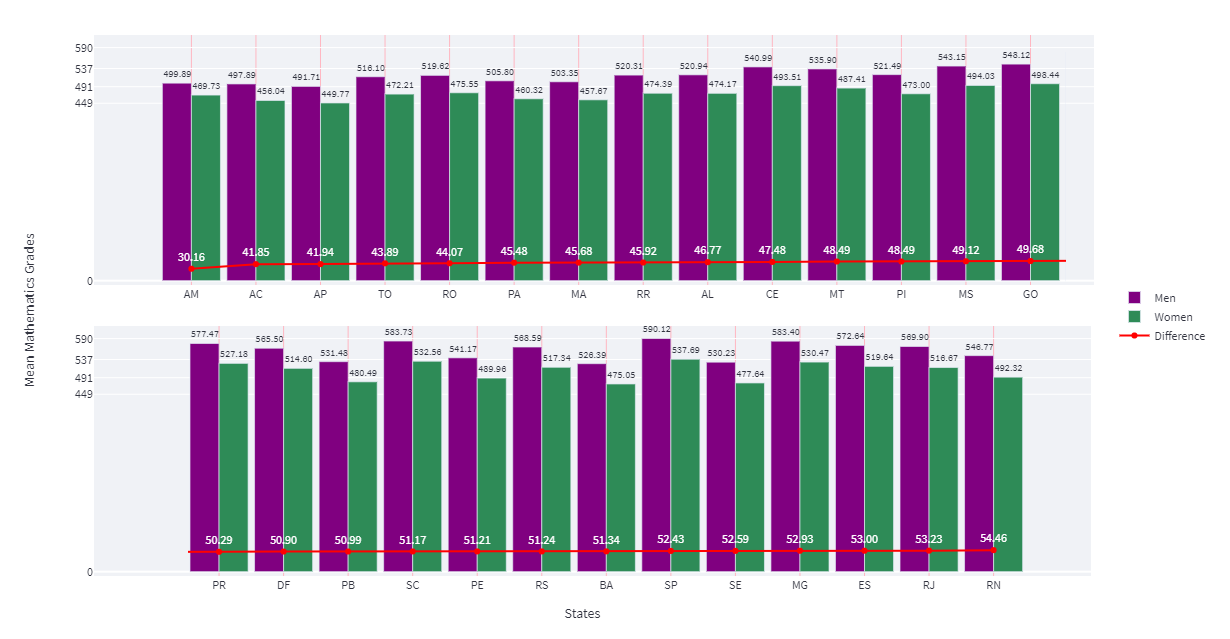
\includegraphics[scale=0.5]{images/mean_math_grades_per_state_and_diff_2020.png}}
\caption{Mean of Mathematics grades per Brazilian State, in 2020.} 
\label{gender}
\end{figure}

In Figure \ref{math_scores}, we show the trend of the average scores of men and women in mathematics over the last six years. It can be seen that both genders had an improvement in performance. However, the difference has widened over the past six years, from  29.08 points in 2015 to 48.33 points in 2020.

\begin{figure}[h!]
\centerline{\includegraphics[scale=0.5]{images/math_scores_by gender_fixed.png}}
\caption{Mean of mathematics grades from 2015 to 2020.} 
\label{math_scores}
\end{figure}

\subsubsection{Analyses by Parents' educational attainment}\

Regarding parents' educational attainment (Table \ref{tab:exTable1}) and parents' profession (Tables \ref{tab:table_fathers_jobs} and \ref{tab:table_mothers_jobs}, shown in next paragraph), we also perceived the impact of these factors in students' performance, as also shown in \cite{Farooq2012FACTORSAS}. Students with parents who had higher educational attainment showed better grades for all the five school subjects in comparison to the ones whose parents had lower educational attainment (Figure \ref{education}). Even though we showed this result using 2020 data, the same pattern occurred for all the range considered in this paper (i.e., from 2015 to 2020, students whose parents had higher educational attainment performed better in all study areas).  


\begin{table}[ht]
\centering
\caption{Parents' educational attainment}
\label{tab:exTable1}
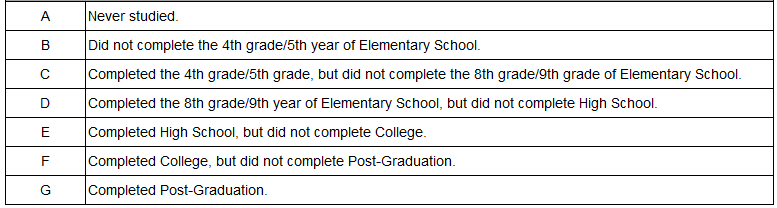
\includegraphics[width=1\textwidth]{images/table_parents_education_level.png}
\end{table}


\begin{figure}[h!]
\centerline{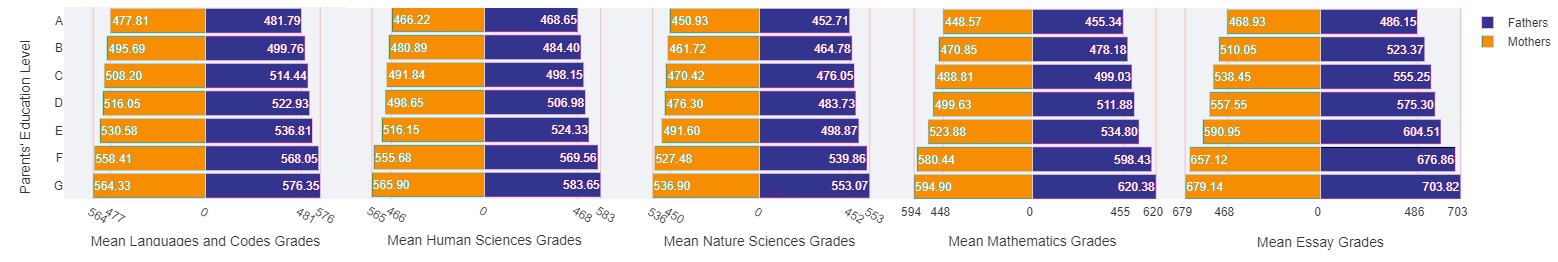
\includegraphics[scale=0.45]{images/mean_grades_per_education_level_2020.png}}
\caption{Mean grades per parents' attainment in 2020.} 
\label{education}
\end{figure}

\subsubsection{Analyses by Parents' profession}

Similarly, students whose parents had less rewarded professions performed worse than the ones whose parents are better rewarded, as we can see in Figure \ref{profession} that shows students' performance in 2020. The same pattern also occurred for all the investigated range (2015-2020) and all school subjects.  

\begin{table}[ht]
\centering
\caption{Fathers' professions}
\label{tab:table_fathers_jobs}
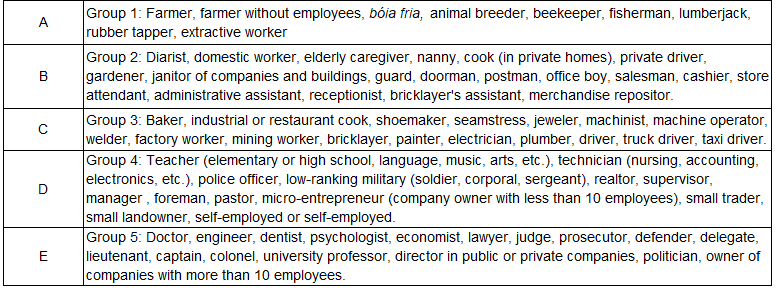
\includegraphics[width=1\textwidth]{images/table_fathers_profession.png}
\end{table}

\begin{table}[ht]
\centering
\caption{Mothers' professions}
\label{tab:table_mothers_jobs}
\includegraphics[width=1\textwidth]{images/table_mothers_profession.png}
\end{table}

\begin{figure}[h!]
\centerline{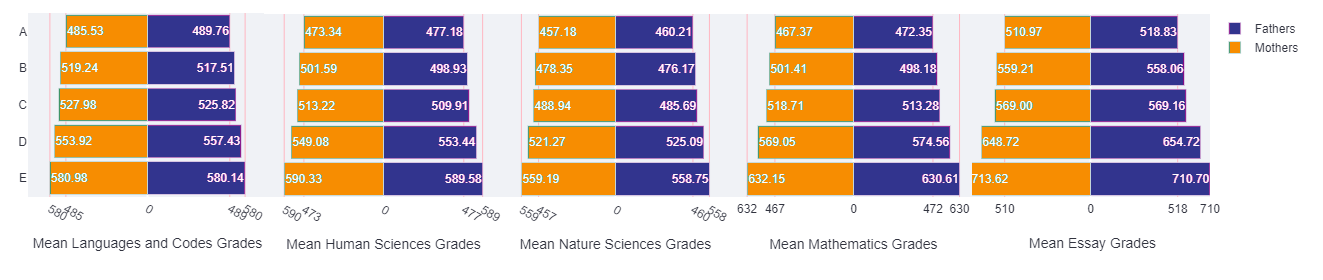
\includegraphics[scale=0.5]{images/mean_grades_per_profession_2020.png}}
\caption{Mean grades per parents' professions, in 2020.} 
\label{profession}
\end{figure}

%Below, we have examples of visualizations provided by our dashboard. 

\subsubsection{Discussion}
% \subsection{Definition of a set of factors from the ENEM dataset} %

Regarding our first research sub-question (RSQ1) that investigates which factors influence the school performance of elementary and high school
students, we can assume we answered it by presenting in our case study the list of factors that impact Brazilian students for the ENEM scenario, which are: 1- parents' educational attainemnt; 2- geographical belongingness; 3- age; 4- gender; 5- marital status; 6- ethnicity; 7- parents' profession; 8- income.

The definition of a set of the most relevant factors that influence student’s performance to be utilized in the data visualization module of our tool was the first result of our work. These factors were utilized to support our analyses.
% (Figure \ref{set_of_factor}) %
Therefore, other researchers can benefit from the use of the set of factors we applied in our case study to replicate similar analyses in the Educational scenario. 

% \begin{figure}[h] \centerline{\includegraphics[scale=0.41]{images/set_of_factors.png}}\caption{Set of factors to be utilized as filters in our analysis.} \label{set_of_factor} \end{figure} %

The answer to our RSQ2 (where we investigate what benefits can the integration of multiple public databases bring to the evaluation of the educational scenario by educational managers) conducted us to our second result, which was the integration of public databases, such as ENEM, and PNAE. We also prepared the data for analysis and visualization phases by preprocessing and cleaning the data, as shown in Section 3.2. 

At last, by answering our third sub-question RSQ3, where we discuss the viability of the creation of a decision support tool to guide Education managers, we reached the last and most important result of this work, which was the design and development of a decision support system that can guide Educational managers in their decision-making process (Figure \ref{dashboard}). 

% \colorbox{green}{[DESCREVER OS RESULTADOS A NÍVEL DE FERRAMENTA? FOI} \colorbox{green}{RÁPIDO A FERRAMENTA? OS GESTORES CONSEGUEM TOMAR DECISÕES?} %

% \colorbox{green}{Quais são as discussões dos objetivos que foram propostos na introdução??} %

\section{Conclusion}

% \colorbox{green}{OS OBJETIVOS FORAM ATENDIDOS? O QUE VOCÊ DESCOBRIU NO ESTUDO?} \colorbox{green}{COMO VOCÊ AJUDOU AOS ENVOLVIDOS? POR QUE SUA PROPOSTA FOI} \colorbox{green}{ IMPORTANTE? QUAIS A LIMITAÇÃO DA SUA PROPOSTA? COMO PODEMOS} \colorbox{green} {SUPERAR ESSAS LIMITAÇÕES?} %
The main goal of this work was the conception of the EduVizBR, an open decision support system designed to assist Education managers in analyzing Brazilian students' school performance.
We conducted our analyses regarding the eight factors defined in our case study (i.e., geographical belongingness, age, gender, marital status, ethnicity, parents' educational attainment, parents' profession, and income). We considered students' performance analyses by gender for all Brazilian states, as well as analyses by parents' educational attainment, and parents' profession. As shown in our case study, we met our expected goals of demonstrating that these factors had some influence in students' performance considering the ENEM scenario.

The EduVizBR can facilitate the decision-making process of Education managers. By using the tool, managers have access to integrated public datasets regarding students' performance and governmental funds data, along with interactive visualizations. The tool proposed in this paper can give insights to the managers about the educational scenario to help them make faster and more reasonable (data-driven) decisions.

We aim to expand our analysis and evolve our tool through the development of the features listed below in our future work.

\subsection{Future Work} 

We are planning on evolving this work mainly by: 
\begin{enumerate}
    \item Providing a mechanism in the EduVizBR that can support the definition of Key Performance Indicators (KPIs) by Education managers. The KPIs will serve as a thermometer to measure whether actions taken in this Education scenario are generating the expected results;
    \item Extending the EduVizBR with a data prediction module that provides Machine Learning algorithms to predict students' performance for the years ahead.
\end{enumerate}

As minor improvements, we aim to compare our findings with the results revealed in the other works from our literature review. Additionally, we will increment our dashboard with a profile of the students who did the ENEM exam, according to sex, age, income, ethnicity, etc.

Finally, we aim to validate our decision support tool using different use cases (other than the ENEM) such as SAEB, ICT Education\footnote{ICT Education available at: \url{https://cetic.br/pt/pesquisa/educacao/}} data, PNAE, and FUNDEB. Using the SAEB data, we aim at analyzing the scores for Math and Portuguese exams of students from elementary and high schools; For the ICT Education data, on the other hand, we plan to analyze the use of technologies in schools over time; and, at last, we plan to analyze the Brazilian investments made in Education over time using FUNDEB and PNAE datasets.

\bibliographystyle{sbc}
\bibliography{sbc-template}

% \section{Appendix} 

% \begin{figure}[h]
% \centerline{\includegraphics[width=\columnwidth]{images/Viz_gender.png}}
% \caption{Mean of Mathematics grades per Brazilian State, in 2018 (This visualization was made using a partition of the 2018 data).} 
% \label{pyramid}
% \end{figure}

% \begin{figure}[h]
% \centerline{\includegraphics[width=\columnwidth]{images/Viz1_mapa.png}}
% \caption{Heatmap showing the distribution of students per Brazilian states in 2018 (This visualization was made using a partition of the 2018 data).} 
% \label{heatmap}
% \end{figure}

% \begin{figure}[h]
% \centerline{\includegraphics[scale=0.8]{images/el_father_0.png}}
% \caption{Parallel graph showing students' grades for the five competences, according to their father education level, in 2018. Here, we highlight the grades for students whose fathers are in the "no study" category. (This visualization was made using a partition of the 2018 data. For axis Y labels, "0" means "no study" and "7" means "post graduation level").} 
% \label{pra_garph_le_father_0}
% \end{figure}

% \begin{figure}[h!]
% \centerline{\includegraphics[width=\columnwidth]{images/el_mother_0.png}}
% \caption{Parallel graph showing students' grades for the five competences, according to their mother education level, in 2018. Here, we highlight the grades for students whose mothers are in the "no study" category. (This visualization was made using a partition of the 2018 data. For axis Y labels, "0" means "no study" and "7" means "post graduation level").} 
% \label{pra_garph_le_mother_0}
% \end{figure}

% \begin{figure}[h!]
% \centerline{\includegraphics[width=\columnwidth]{images/el_father_7.png}}
% \caption{Parallel graph showing students' grades for the five competences, according to their father education level, in 2018. Here, we highlight the grades for students whose fathers are in the "post graduation" category. (This visualization was made using a partition of the 2018 data. For axis Y labels, "0" means "no study" and "7" means "post graduation level").} 
% \label{pra_garph_le_father_7}
% \end{figure}

% \begin{figure}[h!] 
% \centerline{\includegraphics[width=\columnwidth]{images/el_mother_7.png}}
% \caption{Parallel graph showing students' grades for the five competences, according to their mother education level, in 2018. Here, we highlight the grades for students whose mothers are in the "post graduation" category. (This visualization was made using a partition of the 2018 data. For axis Y labels, "0" means "no study" and "7" means "post graduation level").} 
% \label{pra_garph_le_mother_7}
% \end{figure}


% \begin{figure}[h!]
% \centerline{\includegraphics[width=\columnwidth]{images/job_father_0.png}}
% \caption{Parallel graph showing students' grades for the five competences, according to their father profession, in 2018. Here, we highlight the grades for students whose fathers belong to "group 1" category (Farmer, farmer without employees, \emph{bóia fria}, animal breeder, beekeeper, fisherman, lumberjack, rubber tapper, extractive worker). (This visualization was made using a partition of the 2018 data. The labels in axis Y are equivalent to the group to where the fathers belong).} 
% \label{pra_garph_father_job_g1}
% \end{figure}

% \begin{figure}[h!] 
% \centerline{\includegraphics[width=\columnwidth]{images/job_mother_0.png}}
% \caption{Parallel graph showing students' grades for the five competences, according to their mother profession, in 2018. Here, we highlight the grades for students whose mothers belong to "group 1" category (Farmer, farmer without employees, \emph{bóia fria}, animal breeder, beekeeper, fisherwoman, lumberjack, rubber tree, extractive worker). (This visualization was made using a partition of the 2018 data. The labels in axis Y are equivalent to the group to where the mothers belong).} 
% \label{pra_garph_mother_job_g1}
% \end{figure}


\end{document}

